\chapter{AN EVOLUTIONARY ALGORITHM FOR GENERATING PARETO EFFICIENT POTENTIALS}
\label{ch:methodology}

%https://pdfs.semanticscholar.org/3b19/b1f81e1b1a8c28a2f0896b6c84d4c88d57df.pdf
The purpose of this chapter to introduce a cost-efficient algorithm to determine the appropriate tradeoffs in concurrent minimization problems associated with multiple criteria.

In the presence of tradeoffs, the set of Pareto optimal points becomes the solution to minimization with respect to multiple objective functions to be minimized.  We refer to the process of estimating the ensemble of rational potential parameterizations which produce this optimal set as Pareto optimization.   The term ‘rational’ will be discussed in detail, but involves the use of a simple algorithm to identify potential parameterizations that make sense to consider further. This is the central idea of our approach and is very different from a conventional potential fitting approach.

Our algorithm has the following goals: (1) to identify the strengths and weaknesses of alternative parameterizations through analysis of the Pareto optimal solutions, (2) to generate estimates of the Pareto optimal front in a series of iteratively better approximations, and (3) to describe the candidate parameterizations through the use of a distribution function and use of Monte Carlo sampling.  Periodically, the sampling scheme is updated by keeping the Pareto optimal points.  This increases the sampling intensity in the region of parameter space where Pareto optimal points have been identified.

The end state of this algorithm is to a identify the probability distribution which produce Pareto optimal results.  This distribution can be used to integrate this algorithm into existing and well-defined UQ methodologies.  In the development of this evolutionary algorithm, some of the techniques used in genetic algorithims and evolutionary algorithms are consciously not implemented.

\section{Evolutionary Optimization Strategy}
\label{sec:strategy}

%The use of evolutionary strategies in potential optimization was pioneered by Frederiksen \emph{et al.} \cite{fredericksen2004_bayesian_fitting} introduces a Bayesian approach to potential parameterization.
%Neural network approaches were pioneered by Behler and Parrinello \cite{behler2007_NN_potdev} and Sanville \emph{et al.} \cite{sanville2008_NN_potdev_si}.
%Genetic algorithm approach\cite{marques2008_ga_potdev} and \cite{hunger1998_ga_potdev}.

\subsection{Problem Definition}

In taking a new approach to potential optimization, we recall the fundamental challenge, which is the multi-objective optimization problem of minimizing the errors for a large number, $N_Q$, of QOIs. In this case, each objective function is the absolute difference between the predicted material property $\hat{q}_i$, and the target values, $q_i$.  If  $\hat{V}(\bm{\theta})$ is an interatomic potential parameterized by the vector $\bm{\theta} = (\theta_1,...,\theta_{N_P})$ with $N_P$ parameters, then predicted material properties becomes $\hat{\bm{q}}(\bm{\theta}) = (\hat{q}_1,..,.\hat{q}_{N_Q})$.
Using the absolute loss function for our choice of objective functions, the problem then becomes the minimization of  $\bm{L}(\bm{\theta}) = (|\hat{q}_1-q_1|,...,|\hat{q}_{N_Q}-q_{N_Q}|)$, simultaneously.
The optimization problem we thus face is minimizing each objective function in $N_Q$ target properties described by a fixed functional form with $N_P$ parameters.  That is, both error space and parameter space typically have a large number of dimensions.  Here we take the approach of generating a large number of parameter sets through random sampling of the parameter space, and algorithmically determining if these candidate potentials are optimal in a multi-objective optimization sense.  The algorithmic approach we take is centered on the idea of Pareto optimality.  To this multi-objective optimization problem, we can impose both equality and inequality constraints on any parameter $\theta_i$ and inequality constraints on any QOI $\hat{q}_j$.

For a set of $N$ parameterizations of a single potential, denoted $\bm{\Theta}= \{\bm{\theta}_1,...\bm{\theta}_N\}$, a single parameterization $\bm{\theta}_0 \in \bm{\Theta}$ is Pareto optimal if and only if there is no other $\bm{\theta} \in \bm{\Theta}$, such that $|\hat{q}_i(\bm{\theta})-q_i| \leq |\hat{q}_i(\bm{\theta})|$
for all $i<N_Q$, and $|\hat{q}_i(\bm{\theta})-q_i| \leq |\hat{q}_i(\bm{\theta})|$ for at least $i$.  That is, a parameterization $\bm{\theta}$ is Pareto optimal if there does not exist another parameterization which improves performance with regard to one QOI without degrading performance with regard to any another.  Contrariwise, a parameterization is not Pareto optimal if there exists at least one other parameterization which provides a better prediction with respect to predicting one material property without degrading the performance of the any other.

In scalar optimization, there is a unique solution for the global optimization problem.   In the proposed approach, the solution to a multi-objective optimization problem is the Pareto surface.  It identifies Pareto optimal potentials in a $N_Q$-dimensional performance space without explicitly defining a scalar cost function.  Throughout the definition of this methodology, the process was designed to avoid \emph{a priori} assumptions.

%\begin{figure}[ht]
%	\centering
%	\includegraphics{chapter5/img/cost_function_optimization}
%	\caption{Depiction of the the typical approach to optimization.}
%	\label{fig:cost_function_optimization}
%\end{figure}

\begin{figure}[ht]
	\centering
	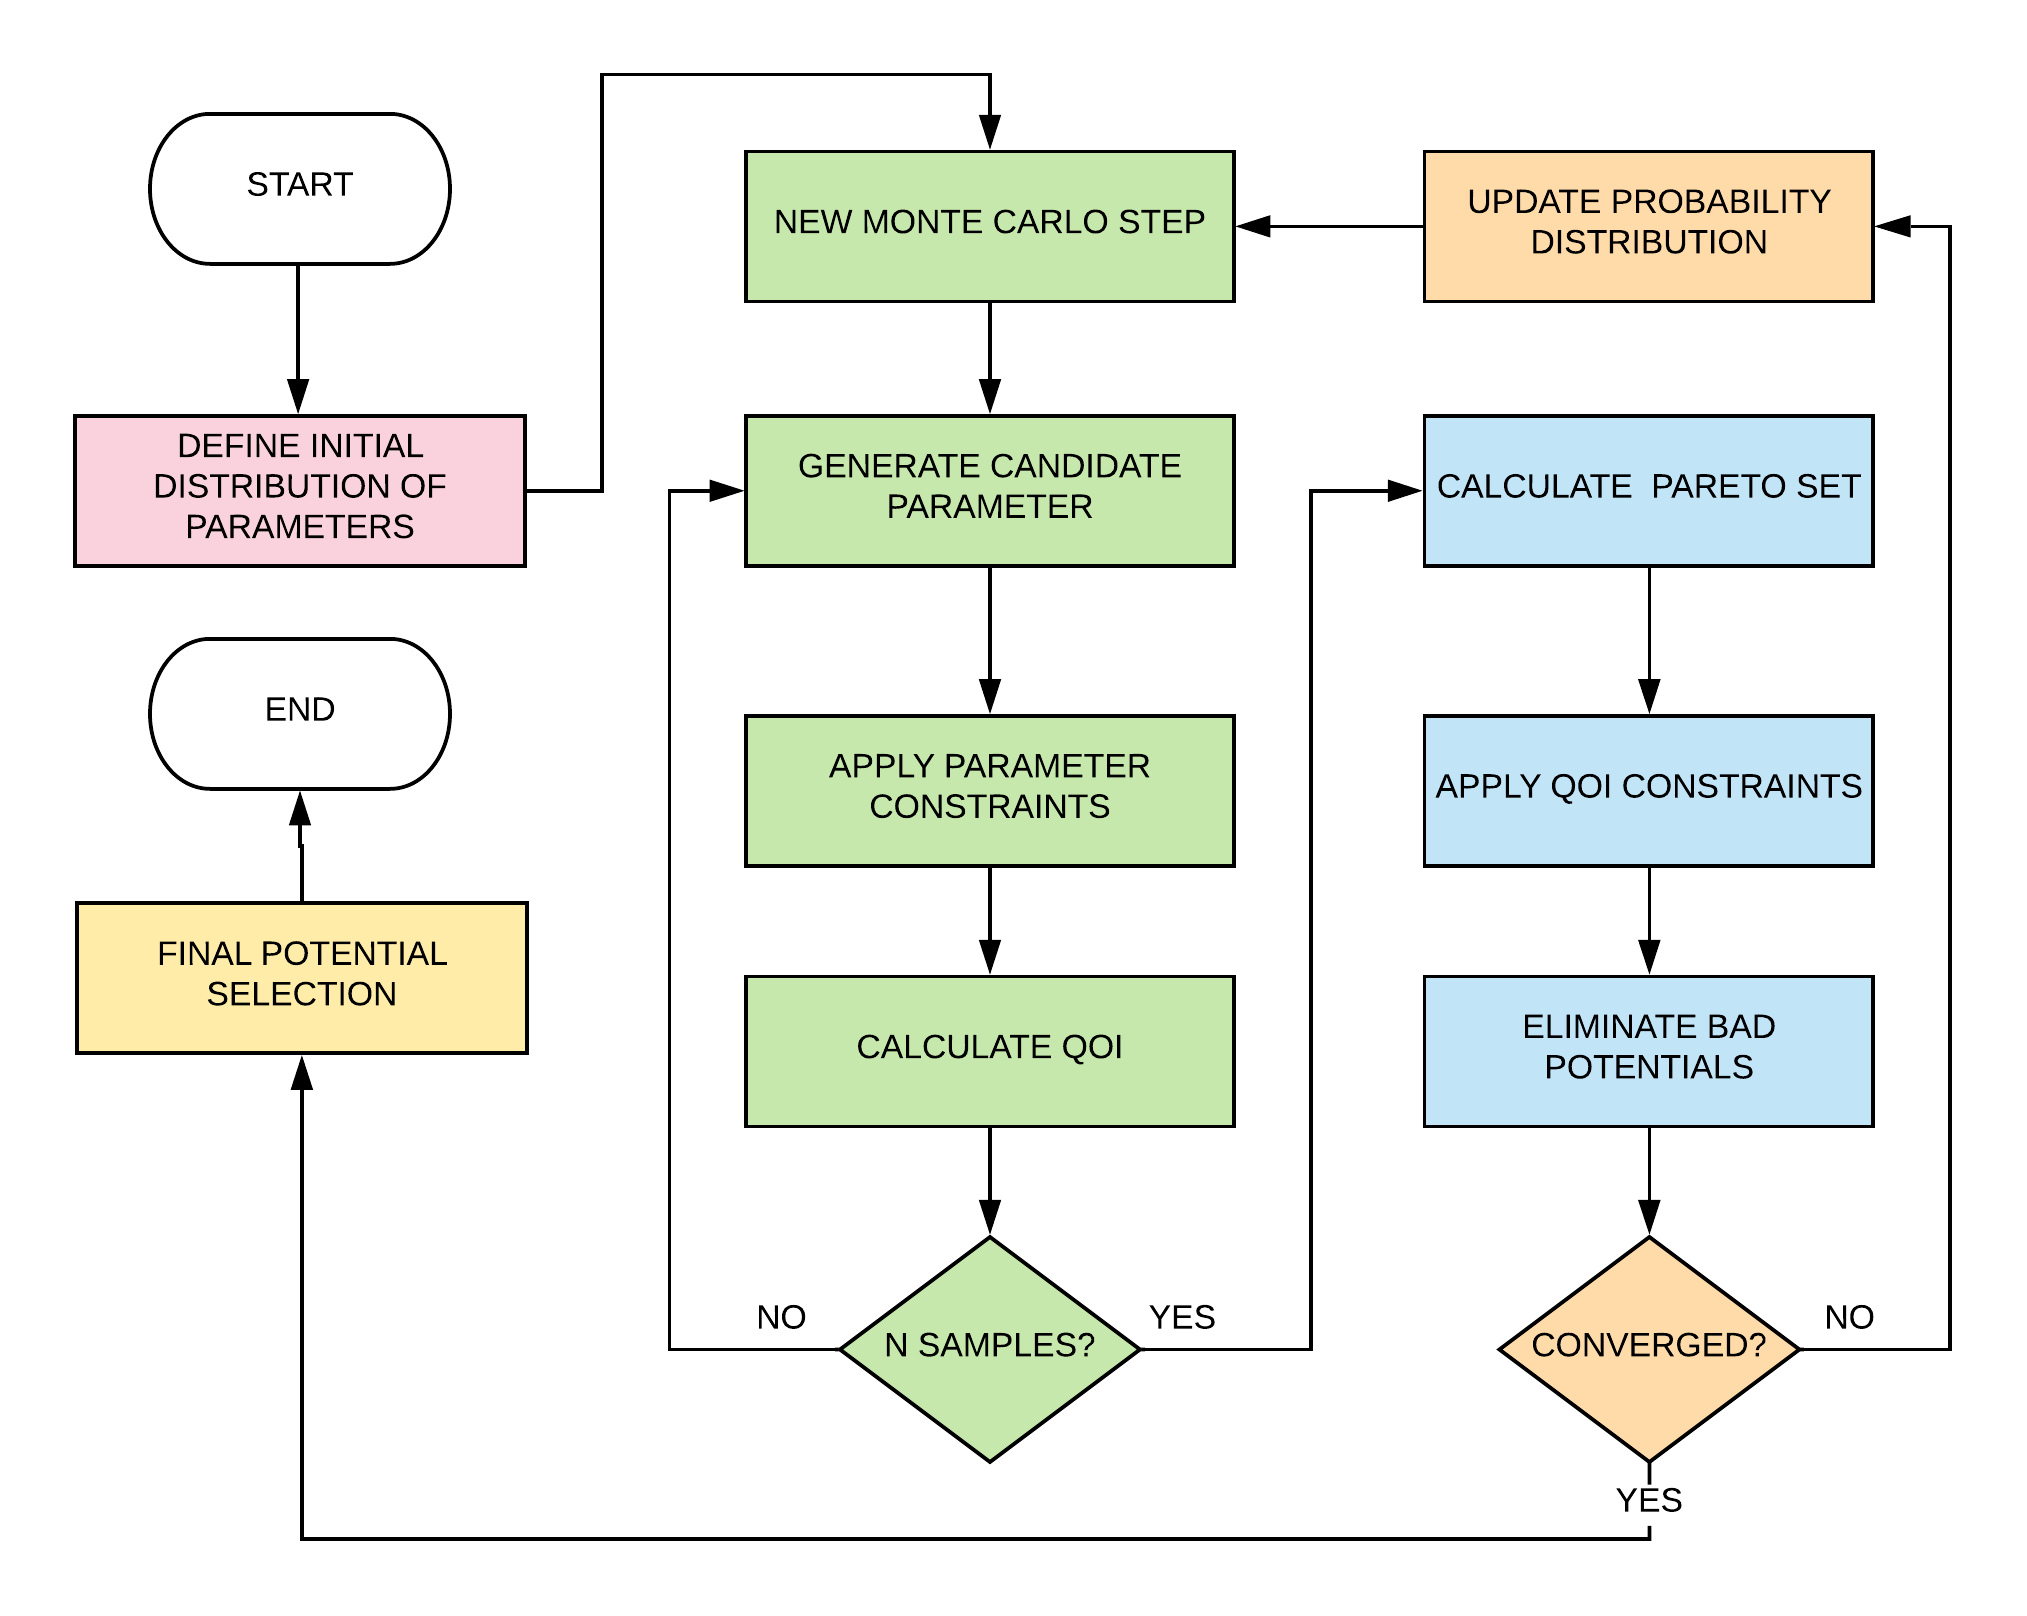
\includegraphics{chapter5/img/pareto_optimization}
	\caption{Schematic of stochastic optimization with Pareto filtering.}
	\label{fig:pareto_optimization}
\end{figure}

We present an optimization scheme that evolves a probability distribution function representing knowledge about the location of Pareto optimal parameters.  As more and better potentials are discovered, the probability distribution function improves the search.  A schematic of the Pareto optimization strategy is depicted in Figure \ref{fig:pareto_optimization}.  This technique is iterative; initial conditions are determined and a series of optimization steps are taken until a convergence condition is met.  Since this process produces an ensemble of potentials, a method of potential selection now occurs.

The red component in Figure \ref{fig:pareto_optimization} is the initial problem definition and incorporation of prior knowledge.  This step consists of the problem definition for parameter optimization.  The scalar optimization of a cost function is replaced with a multi-objective optimization problem.  While scalar optimization results in a single potential $\bm{\theta}^*$, the solution of a MOO problem are the Pareto set $\bm{\Theta}^*$.  Implicit in this process is the identification of structures, properties, and target values which are used in potential fitting. The specific values can be taken from experiment, from higher fidelity calculation methods such as quantum chemical or density functional theory (DFT) calculations, or a combination thereof. Our approach in this step is similar to standard potential development approaches, as discussed in Chapter \ref{ch:potential_development}.  In this approach, a \emph{prior} distribution expressing the uncertainty about the distribution of parameters is defined as starting condition.

The green components of Figure \ref{fig:pareto_optimization} are representative of a Monte Carlo scheme.  Here parameter constraints are applied either by calculation, in the case of equality constraints, or a simple acceptence/rejection mechanism to enforce inequality constraints.  If a generated potential parameter set violates any of the constraints, it is rejected.  Acceptable parameters are then sent to a simulation process which produces predictions on material properties, referred here to as quantities of interest (QOIs).  This process is modeled here as a black box function. These are the set of simulations, as discussed in Chapter \ref{ch:potential_development}.  A framework for implementing the calculation of the QOIs is discussed in Chapter \ref{ch:software}.

The blue components filter the results from the Monte Carlo scheme to provide the optimized results for that iteration.  Dominated points are removed to insure the final set of candidate parameters are a set of Pareto optimal potentials.  Performance filters are applied to satisfy constraints on prediction of material properties.  The last filter proposed removes potential candidates that survive the first two filters, but produce pathologically poor predictions.

The orange components of Figure \ref{fig:pareto_optimization} updates the sampling probability distribution.  A non-parametric probability density function provides more flexiblity than standard parametric probability density functions, which have strong \emph{a priori} assumptions on the underlying distribution.  With a more refined probability distribution function to represent the potential parameters, the prior distribution is updated and a new iterative step can proceed.  To terminate the iterative loop, the algorithm can either continue for a fixed number of iterative steps or until a convergence condition is met.

The yellow component in Figure \ref{fig:pareto_optimization} is the potential selection process.  Unlike the methods discussed in Chapter \ref{ch:potential_development}, this method produces an ensemble of possible parameterizations.  All these potentials meet our criteria: they are Pareto optimal and satisfy constraints on the potential parameters and QOI predictions; any of these potentials can be rationally chosen.  At this point, the selection of potentials becomes subjective.  However, the potential developer can make a more informed decision based upon the tradeoffs available.  Scoring functions are introduced here to simplify analysis.

\subsection{Structure of this Chapter}

The remainder of Section \ref{sec:strategy} provides a broad overview of this algorithm and compares it to the scalar optimization approach presented in Chapter \ref{ch:potential_development}.  While the two approaches have similar process analogues, the typical potential development technique is a deterministic optimization problem; ours is a stochastic process.

Section \ref{sec:probability} starts with a discussion of probability and random variables.  This methodology uses the ideas and methods from a wide rage of probability methods, such as Monte Carlo sampling, Bayesian analysis and uncertainty quantification.  This section introduces notation and terminology and has been adapted for our problem context.

Section \ref{sec:prior_information} incorporates incorporation of prior information before starting the potential optimziation procedure.  Topics such as the selction of the fitting database, the application of constraints on both potential parameters and predictions of material properties were discussed extensively in Chapter \ref{ch:potential_development}.  As a result, this section focuses on the definition of \emph{prior} distribution, which is the initial probability distribution function which will be evolved through sampling and analysis to update the prior distribution iteratively.

Section \ref{sec:sampling} deals with process of sampling parameters $\bm{\theta}$ from a defined probability distribution.  These potential parameterizations ($[\bm{\theta}_1,...,\bm{\theta}_N]$) are set of predictions can be acquired $[\hat{\bm{q}}(\bm{\theta}_1),...,\hat{\bm{q}}(\bm{\theta}_N)]$. This approach is typical of Monte Carlo solution techniques.

Section \ref{sec:filtering} discusses the application of a variety of filters to determine the optimal candidate potentials.  The predominant feature of this methodology is the Pareto filter, but other filters eliminate candidate potentials which violate inequality constraints on predicted material properties.  Additionally, as the number of Pareto optimal candidates increases, the new potential identification becomes more difficult.  To reduce sampling dispersion, a filter to eliminate pathological potentials is devised; this improves sampling in the region of interest by concentrating sampling in the region of the surviving potentials and reduces dispersion due to the spread of the correlation matrix.

Section \ref{sec:iterative_loop} defines the iterative loop by updating the prior distribution used for sampling parameter space. A non-parametric probability density function provides more flexibility over standard parametric distribution function. Issues involving convergence of the probability density function as a stopping condition are also discussed in this section.

Section \ref{sec:selection} discusses of down selection and selection techniques.  Since chapters proceeding this chapter discusses the selection of rational potentials in more detail, this discussion here is cursory.

\section{Probability}
\label{sec:probability}
What follows is a necessarily brief introduction to probability theory.  For a more rigorous approach, the classic textbooks of Rudin\cite{rudin1987_realanalysis} for a treatment of measure theory and Chung\cite{chung2001_probabilitytheory} for a measure theory construction of probability are recommended.

Let $(\Omega,\mathcal{F},\mathbb{P})$ be a measure space with $\mathbb{P}(\Omega)=1$.  Then $(\Omega,\mathcal{F},\mathbb{P})$ is a probability space, with sample space $\Omega$, event space $\mathcal{F}$, and probabilty measure $\mathbb{P}$.  The underlying foundation of any probability distribution is the sample space, which is the set of all probable outcomes denoted as $\Omega$.  The realization of an outcome is denoted $\omega \in \Omega$.

The events for the measure space are defined in such a way that a probability measure can be assigned.  This allows the assignment of probability measures on complex events to characterize groups of outcomes.  The collection of all such events is a $\sigma$-algebra $\mathcal{F}$ of subsets of $\Omega$.  Not every subset of the sample space $\Omega$ must be considered an event, the $\sigma$-algebra restricts $\mathcal{F}$ to subsets of $\Omega$ for which $\mathbb{P}$ can be asssigned.

The probability measure, $\mathbb{P}$, is a function which maps $\mathbb{P}:\mathcal{F}\rightarrow[0,1]$.  A probability is a real number between zero and one.  Within this work, we do not distinguish between impossible events which have probability zero, and probability-zero events which are not necessarily impossible.  Events of probability one happens almost surely, with almost total certainty.

\subsection{Random Variables}

A random variable $X$ is a variable whose possible values are outcomes of random phenomena.  As a function, a random variable is required to be measurable, which rules out pathological issues.  The probability measure $\mathbb{P}$ assigns probabilities for a random variable $X$ over the possible values $x \in X$.  Specifically, $X:\Omega\rightarrow\mathbb{R}$.  If a random variable $X:\Omega \rightarrow \mathbb{R}$ is defined on the probability space $(\Omega,\mathcal{F},\mathbb{P})$, then the probability of an event $A$ occuring is $\{\omega:X(\omega)=A\}$ which is denoted as $\mathbb{P}(X=A)$.

Formally, a random variable is a particular type of measurable function.  However, there is an important difference which may be more philosophical than mathematical due to the difference in the underlying domains.  A random variable operates on a set of outcomes or processes defined by $\Omega$, while deterministic variables does not.  This isn't a mathematical difference, as the underlying domains are just sets, and the $\sigma$-algebra and measures provide the relevant mathematical structure.

For a probability space, even if a specific random process isn't mentioned, there is an implied assumption that such a random process exists.  Otherwise, there would be no need for probability to have its own language.

A random variable is evaluated by performing an unpredictable experiment.  That is, one in which $\omega \in \Omega$ is not predetermined.  The selection of a specific $\omega$, isn't the evaluation of a random variable, it is simply the evaluation of a measurable function.  We denote the realization of a random variable as $x(\omega) \in X(\Omega)$, to differentiate from the deterministic elements of a set, which uses the $x \in X$ notation.


\subsection{Probability Density Functions}

In the potential optimization process, the potential parameters are modeled as random variables.  This is denoted $\bm{\theta}(\omega_i) \in \bm{\Theta}(\Omega)$ with $\omega \in \Omega$.  The random variable $\bm{\Theta}(\Omega)$ has specific realizations $\bm{\theta}(\omega)$ on the event space $\omega \in \Omega$ with probabilities determined by the probability measure $\mathbb{P}$.
Since a specific outcome $\omega_i$ produces $\bm{\theta}$, $\bm{\theta}_i=\bm{\theta}(\omega_i)$ is no longer probabilistic, but deterministic.  Thus, $N$ candidate parameterizations generated from $\bm{\Theta}(\Omega)$ can be denoted as a set of $N$ constant vectors,
$
 \{\bm{\theta}(\omega_1),...,\bm{\theta}(\omega_N)\}
=\{\bm{\theta}_1,...,\bm{\theta}_N\}
=\bm{\Theta}
$.  In this work, the $\omega$ notation usually indicates simulations to be done that still need to be realized, and the lack of of an $\omega$ notation indicates that the simulation have already been done.

If $\bm{\Theta}(\Omega)$ is a random variable with a finite number of outcomes, then the sequence of $\{\bm{\theta}_1,...,\bm{\theta}_N\}$ occurs with the probabilities $\{p_1,p_2,...p_k\}$, and $\mathbb{P}(\bm{\theta})=p_{\Theta}(\bm{\theta})$ is a \emph{probability mass function}.
To simplify notation, $p_\Theta(\bm{\theta})=p(\bm{\theta})$ omits the subscript $\Theta$ since $\bm{\theta}\in\bm{\Theta}$ implies it.

A continuous random variable $\bm{\Theta}(\Omega)$ admits the \emph{probability density function} $p_{\Theta}(\bm{\theta})$. The probability density function is used to compute probabilities over ranges of values. The probability of an event $\bm{\Theta}' \subseteq \bm{\Theta}$ occuring is defined by the integral.
\begin{equation}
	\label{eq:continuous_random_variable}
  \mathbb{P}(\bm{\Theta}=\bm{\Theta}')
	=
	\int_{\theta \in \Theta'} p_{\Theta}(\bm{\theta}) d \bm{\theta}.
\end{equation}
For continuous random variables, the probability of a specific event happening $\mathbb{P}(\theta(\omega))$ is vanishingly small.  Since the bounds of integration on Equation \ref{eq:continuous_random_variable} vanish,  $\mathbb{P}(\bm{\theta}(\omega))=0$, almost surely.  The probability density function (PDF) still remains an expression of likeliness.
If $p(\bm{\theta}_1)>p(\bm{\theta}_2)$, then $\bm{\theta}_1$ is more likely to happen than $\bm{\theta}_2$.

 The expectation of a random variable $\mathbb{E}$ is the average of the outcomes weighted by their probability mass function or probability density function.  For discrete random variables,
 \begin{equation}
	 \mathbb{E}[X] = \sum_{x\in X} x p(x).
	\end{equation}
For continuous random variables, this summation becomes the
\begin{equation}
	\mathbb{E}[X] = \int_{-\infty}^{+\infty} x p(x) dx
\end{equation}
The expectation of a function $f$ dependent upon a random variable $X$ can likewise be defined as
\begin{equation}
	\mathbb{E}[f(X)] = \int_{-\infty}^{+\infty} f(x) p(x) dx
\end{equation}
\subsection{Monte Carlo Methods}
Monte Carlo methods\cite{thomopoulos2013_montecarlo} are a broad class of computational algorithms which are dependent upon random sampling to obtain numerical results.
The essential aspect of these approaches is to use randomness to solve problems which might be deterministic in principle.
Monte Carlo simulations sample from a probability distribution for each variable to produce an arbitrarily large number of possible outcomes; the results are analyzed to get probabilities of different outcomes occuring.  The process for generating random samples from a probability distribution function is discussed more thoroughly in Section \ref{sec:sampling}.

In scalar optimization problems, random sampling methods are ubiquituous for global minimization, including techniques such as simulated annealing\cite{kirkpatrick1983_simmulated_annealing}, genetic algorithms\cite{holland1975_ga}, and tabu search\cite{glover1986_tabu}.  Although these approaches require a large number of samples, they do not require \emph{a priori} knowledge of the objective function to achieve the global mimima.
Here we take the approach of generating a large number of parameter sets through random sampling of the parameter space, and then algorithmically determining if the set of candidate potentials are optimal in the multi-objective context.  The algorithmic approach we take is centered on the idea of Pareto optimality.

\subsection{Interpretation of Probabilities}

The meaning of the probabilities assigned to potential values of a random variable $\bm{\Theta}(\Omega)$ is not related to probability theory itself, but instead related to philosophical context over the interpretation of probability.  In most scientific applications, the probability interpretation is physical in nature, in which probabilities are objective and an event's probability is the limit of its relative frequency as the number of samples becomes large.  This interpretation supports the statistical needs and inference requirements for experimental scientists since probabilities can be found by a repeatable objective process (e.g. experiments), and are thus devoid of opinion.  Within this context, probabilities are \emph{aleatory}.  Uncertainty is irreducible and inherent to to the physical process observed.

For finite temperature simulation above $0$ K, molecular dynamics simulations allow sampling from themodynamic ensembles.  Although the simulations are replicable since time-integration and the empirical potential are deterministic, sampling from the time-series or by randomly assigning initial velocities, allows molecular dynamics to model the aleatory uncertainty associated with a $T > 0$ K simulations.

Within the context of potential development, probabilities are evidentiary and can be assigned to any problem statements even through no random process is involved, as a way to represent subjective plausibility, or to the degree in which the statement is supported by available evidence.  Evidential probabilities represent degrees of belief, such as the Laplace interpretation where probabilities are defined in the disposition to gamble at certain odds\cite{laplace1902_probability}.  These coherent subjective belief systems follow the laws of probability\cite{ramsey2016truth,definetti1980_foresight}.  Here, uncertainty is \emph{epistemic} and is based on current evidence, but is mutable based upon receiving new observations\cite{ramsey2016truth,definetti1980_foresight,jaynes2003_probability}.  This philsophical interpretation is more closely associatiated with Bayesian inference\cite{gelman_bayesian}.

In practice, the uncertainty associated with any problem has both \emph{aleatory} and \emph{epistemic} components.  Within this context, the field of uncertainty quantification\cite{oberkampf2010_vvuq} is involved with the quantitative characterization and reduction of uncertainties in both computational and real world applications.  The difficulty of applying Bayesian frameworks to potential development is constrained to the size of the training dataset and the biases produced in assigning preferences due to the inevitable tradeoffs in material properties prediction.  Moreover, the inability to define uncertainities associated with target properties in a meaningful probabilistic sense frustrates standard VVUQ and Bayesian approaches.

\section{Incorporation of Prior Information}
\label{sec:prior_information}

All iterative techniques have initial starting conditions.  In a deterministic method such as scalar minimization using gradient descent techniques, the starting conditions are the initial estimate of the solution.  In our case, the location of the best estimate may not be known; the initial condition requires not only an expression of location but also of range.  Bayesian techniques refer to this process as the definition of the prior distribution.  Here, we generalize this concept by not only defining the prior distribution, but also constraints on the potential optimization problem.

For existing formalisms, one can incorporate parameter information from existing potentials.  For each parameter, define an uppper and lower bound to define the uniform distribution.  Having a uniform prior means that the probability density is constant over its support, defined as $\theta_{i}^{\text{min}} \leq \theta_i \leq \theta_{i}^{\text{max}}.$  A uniform prior doesn't favor any particular value of $\theta_i$, since it supposes that all values in the range are equally likely.  This is referred to in Bayesian literature as a \emph{vague} or \emph{uninformative} prior.  Strictly speaking, the use of uniform priors are optimal since an uniformative prior information for $\bm{\theta}$ must be identical over its support.    However, complete ignorance about the distribution of a potentials parameter may not be true.

Based upon application, different probability distribution functions can be selected to represent prior knowledge.  The starting condition for Pareto analysis could be based upon the existing parameterization, $\bm{\theta}_0^*$, of a potential formalism.  This optimization choice is based upon a set of undocumented optimization conditions, such as optimization method, the choice of weighting vectors of the cost function, $C(\bm{\theta}|\bm{w})$, and the initial starting condition, $\bm{\theta}_0$.  In this case, the potential developer may be interested in a Pareto analysis of the local energy basin in the neighborhood of  $\bm{\theta}_0^*$.  Sensitivity analysis evaluates changes in the predictive performance of a potential caused by perturbations on $\bm{\theta}_0^*$.  Since a potential developer would never rationally choose a potential that was not Pareto optimal, it is desirable to impose the restriction that changes in potential parameterization must remain Pareto efficient.  A probabability distribution such as the multivariate normal distribution could be selected with the mean vector equal to $\bm{\theta}_0$ to localize the region of sampling.  To disperse the sampling around the mean, the choice of a covariance matrix $\bm{\Sigma}$ is necessary.  A covariance matrix can be defined with $\bm{\sigma}_{\theta_i}$ for the diagonal elements.
Here specifying $\bm{\mu} = \bm{\theta}_0$ encodes prior information about the location of Pareto optimal potentials, while the uncertainty of $\bm{\Sigma}$ remains subjective.  For each $\theta_i$, the potential developer encodes the \emph{epistemic} uncertainty associated with $\theta_i$ with $\sigma_i^2$.

The choice of the \emph{prior} distribution is not important other than it encompasses the region of interest without making the sampling region excessively large.  If the sampling region is too large, then Monte Carlo sampling will produce undesirable \emph{discrepancies} in the sampling sequence; the sequence of random variates will fail to adequately fill the probability space.

In this methodology, potential development is iterative.  To save computational resources, we can identify a set of potentials that meet a small subset of desirable conditions, such as the cohesive energy $E_c$ and the lattice parameter $a_0$ being close to the reference values, $q_{E_c}$ and $q_{a_0}$ respectively, without the constraints of Pareto optimality.  We call this process \emph{pre-conditioning} as it provides enough data points to avoid catastrophic simulation failure due to an ill-conditioned covariance matrix.  Here, the entire population is used as an expression of the prior distribution and can be used to estimate a parametric probability distribution or used to define a non-parametric probability distribution.

\section{Sampling from the Prior Distribution}
\label{sec:sampling}

\subsection{Sampling distribution}

The sampling distribution, $p(\hat{\bm{q}}|\bm{\theta})$, is the distribution of the QOIs conditioned upon the prior distribution $p(\bm{\theta})$.  Instead of analytically determining $p(\hat{\bm{q}}|\bm{\theta})$ and sampling from it, we note that $\hat{\bm{q}}(\bm{\theta})$ is a deterministic function.  As a result, the random variable $\hat{\bm{Q}}(\Omega)$ is a function dependent upon upon $\bm{\Theta}(\Omega)$, which we will exploit as an alternative method of sampling from $\hat{\bm{Q}}(\Omega)$.  We now proceed to outline the process for sampling from $\hat{\bm{Q}}(\Omega)$.

First, generate $\bm{\theta}(\omega_1) \in \bm{\Theta}(\Omega)$, using the prior distribution described in Section \ref{sec:prior_information}.  For a simulation length of $N$, then random variates of potential parameterizations are the independent samples $\{\bm{\theta}(\omega_1),...,\bm{\theta}(\omega_N)\}$ with $\omega_i \in \Omega$ to define the sequence
\begin{equation}
\label{eq:theta_seq}
	  \bm{\Theta} = \{\bm{\theta}_1,...,\bm{\theta}_N\}
\end{equation}

To sample from $p(\hat{\bm{q}}|\bm{\theta})$, the sequence defined in Equation \ref{eq:theta_seq} is evaluated through simulation machinery to calculate
\begin{equation}
\label{eq:qoi_seq}
	\hat{\bm{Q}}
	= \hat{\bm{Q}}(\bm{\Theta})
	= \{\hat{\bm{q}}(\bm{\theta}_1),...,\hat{\bm{q}}(\bm{\theta}_N)\}
\end{equation}

To show that sequence $\bm{Q}$ is generated from $\hat{\bm{Q}}(\Omega)$, consider that each $\bm{\theta}_i$ is a specific realization from $\bm{\Theta}(\Omega)$ with $\omega_i \in \Omega$.
For each $\hat{\bm{q}}(\bm{\theta}_i)$,
\begin{equation}
	\hat{\bm{q}}(\bm{\theta}_i) = \hat{\bm{q}}(\bm{\theta}(\omega_i)) = \hat{\bm{q}}(\omega_i) \in \hat{\bm{Q}}(\Omega)
\end{equation}
with $\omega_i \in \Omega$.

\subsection{Enforcement of Parameter Constraints}

The process of sampling makes the application of parameter constraints trivial.  Equality and inequality constraints are the two classes of potential parameter constraints which have to be enforced.

The enforcement of the inequality constraint $g_{\theta}$ on the parameter $\theta \in \Theta$, imposes $p(\theta_i)=0$ for every $\theta_i$ which violates $g_{\theta}$.  Instead of analytically modifying the prior distribution, an acceptance/reject mechanism is implemented.  For a parameter set $\bm{\theta}_j$, the parameter set is rejected and not included in $\bm{\Theta}$ when if $\theta_{ij}$ violates $g_{\theta}$,

Equality constraints on the parameter $\bm{\theta}_i$ is a function $h_{\theta_i} (\{\bm{\theta}_j; i \neq j\},A)$ where $\{\bm{\theta}_j; i \neq j\}$ are remaining parameters and $A$ is a constant.  To prevent simulation failures, equality constraints should always be imposed explicitly.  Random variates of the free parameters are generated.  Evaluating the function $h$ calculates the equality constrained parameter directly.

Since our proposed process uses a Monte Carlo sampling strategy, the implementation of parameter constraints only requires the definition of constraints as fully determined function of the free parameters.  In the conventional approach of described in Chapter \ref{ch:potential_development}, constraints by implementing either an approximating simplex algorithm.  For exact solutions, non-linear programming strategy must be devised, and the becomes NP-hard when $\hat{\bm{q}}(\bm{\theta})$ is convex\cite{bertsekas1995_nlp}.

\subsection{Generation of Random Variates}
\label{sec:generating_random_variates}

The generation of random variates from a probability distributon is a well-defined process, provided in many statistical software libraries.  However, this approach does present some computational challenges due to numerical stability, which are addressed here.

The commonly used technique to generate random variates of a random variable with a probability distribution function is the inverse transform method.

Let $U(\Omega)$ be a uniform random variable in the range $[0,1]$.  For the potential parameter $\theta(\omega) \in \Theta(\Omega)$ with the probability density function $p_\Theta(\theta)$, the monotonically increasing cumulative density function can be defined,
\begin{equation}
	  F(\theta) = \mathbb{P}(\Theta < \theta) = \int_{-\infty}^\theta p_\Theta(x) dx
\end{equation}

The random variable $\Theta(\Omega)$ can now be defined as a function of the $U(\Omega)$, $\Theta(\Omega)=F^{-1}(U(\Omega))$.  Therefore, if we have a random number to generate numbers according to the uniform distribution, we can generate any random variable with a known probability density function.

The generating of random variates for multivariate probability density functions is considerably more complicated since the the cumulative density function has no mulitvariate analog.  More typically, for multivariate Monte Carlo sampling schemes, the choice of the prior distribution must be some transformation of the multivariate normal distribution, which has convenient mathematical properties\cite{devroye1986}.

The generation of draws from a univariate normal distribution $y \in N(\mu,\sigma^2)$ can be done from the rescaling of a standard normal distribution $x \in N(0,1)$ by the transformation
\begin{equation}
\label{eq:normal_scaling}
	  y = \mu + \sigma x
\end{equation}
which is dependent upon a high quality method to draw a simulated $N(0,1)$, which is a mature technology.

The multivariate normal distribution (MVN) is defined by $\bm{\mu}$ and covariance matrix $\bm{\Sigma}$.
Since  $\sigma_{ij}=\sigma_{ji}$, $\Sigma$ must be symmetric.  The necessity for the MVN having a positive definite covariance matrix comes from its probability density functions.
\begin{equation}
	  p_{\mathrm{MVN}}(\bm{x})
		=
		\frac{1}
		     {(2\pi)^{1/2} |\bm{\Sigma}|^{1/2} }
		\exp\left( -\frac{1}{2} (\bm{x}-\bm{\mu})^T
		                        \bm{\Sigma}^{-1}
														(\bm{x}-\bm{\mu})\right)
\end{equation}
which requires invertibility of the covariance matrix.

% https://crmda.dept.ku.edu/guides/42.mvn/mvn-generator-1.pdf
The multivariate version of the rescaling described in Equation \ref{eq:normal_scaling} is described in Scheuer and Stoller\cite{scheuer1962_mvn_rv}, which is the predominant implementation of generating random variates in statistical software.  A vector $\bm{x}$ of $N$ values is drawn from an $\mathrm{MVN}(\bm{0},\bm{I})$ process.  Setting the mean vector $\mu$ to $\bm{0}$ centers the distribution at $\bm{0}$.
Settting the covariance matrix $\bm{\Sigma}$ to the identity matrix $\bm{I}$, ensures that every component of $\bm{x}$ is independent from each other since all off-diagonal terms are set to zero.  The multivariate standard normal distribution is equivalent to stating that each element of $\bm{x}$ can be drawn independently from $x_i \sim N(0,1)$.
We want to apply a transformation so that the result is $\bm{y} \sim \mathrm{MVN}(\bm{\mu},\bm{\Sigma})$.  This transformation is $\bm{y}=\bm{\mu} + \bm{S} \bm{x}$ where $\bm{S}$ is a square scaling matrix.  $\bm{S}$ has the same purpose that $\sigma$ has in Equation \ref{eq:normal_scaling}.
If the scaling matrix is chosen so that $\bm{\Sigma}_Y = \bm{S}\bm{S}^T$, this transformation produces the correct expectations
\begin{equation}
	  \mathbb{E}[\bm{y}]
		= \mathbb{E}\left[\bm{\mu} + \bm{S}\bm{x}\right]
		= \bm{\mu} + \bm{S} \mathbb{E}[\bm{x}]
		= \bm{\mu}
\end{equation}
the covariance matrix of $\bm{y}$ is
\begin{equation}
	\bm{\Sigma}_Y
	= \bm{S} \bm{\Sigma}_X \bm{S}^T
	= \bm{S} \bm{I} \bm{S}^T
	= \bm{S}\bm{S}^T
\end{equation}
To establish that $\bm{y}$ is an MVN from this transformation, any linear fuction of a vector of jointly normally distributed variables is also normally distributed\cite{greene2003}.  Thus, for $\bm{x} \sim N(\bm{\mu},\bm{\Sigma})$,
\begin{equation}
    \bm{A} \bm{x} + \bm{b}
		\sim N(\bm{A} \bm{\mu} + \bm{b},
		       \bm{A} \bm{\Sigma} \bm{A}^T)
\end{equation}

In the univariate case, $\sigma$ is the square root of the variance $\sigma^2$.  The variance is a parameter of the normal distribution, and $\sigma$ is a derived quantity and could have taken either a negative or positive value.  Since in Equation \ref{eq:normal_scaling} we interpret $\sigma$ to be the standard deviation of a variable, we choose $\sigma > 0$.  Likewise, matrix square roots are grossly different from each other, and there are many approaches known as matrix decompositions to determine them.  In many statistical packages, the Cholesky decomposition of $\bm{\Sigma}$ is calculated to find an lower triangular matrix $\bm{L}$ so that $\Sigma = \bm{L}\bm{L}^T$\cite{golub1996_matrices}.

Since $\bm{\Sigma}$ is positive definite, then all of the eigenvalues of $\bm{\Sigma}$ are greater than zero.  However, an eigenvalue which is 0 or a small positive number can lead to a negative number due to truncation error in numerical routines.  For random variate methods depending upon the Cholesky decomposition, this leads to catastrophic failure of the generation of samples dependent upon generating random variates of the MVN.  For our methodology, later iterations are dependent upon drawing samples from the the MVN.  To correct this problem, the eigenvalue decomposition on $\bm{\Sigma}$ is calculated to check that $\bm{\Sigma}$ is positive semi-definite by inspection of the eigenvalues.  If the eigenvalue is tolerably negative, that eigenvalue is either set to $0$ or a sufficiently small number, and the modified covariance matrix is used.

Accounting for the equality constraints requires modification of the sampling procedure.  If $\bm{\theta}_i$ is a linear combination of other potential parameters, then the underlying covariance matrix will be rank deficient.  By definition, an equality constraint imposes a correlation coefficient of unity to an off-diagonal term, which prevents the Cholesky decomposition of the covariance matrix.  The problems of rank deficiency of the correlation matrix is avoided by evaluating equality constrained potential parameters by direct evaluation of the constraining function after the unconstrained potential parameters have been generated.

\section{Filtering Simulation Results}
\label{sec:filtering}

The final step in the Bayesian process is determination of the posterior distribution.  The posterior distribution is the distribution of the parameters $p(\bm{\theta}|\hat{\bm{q}})$ after taking to account the observed data.  In the deterministic approach, the deterministic approach outlined in Chapter \ref{ch:potential_development}, $\bm{\Theta}^*$ is the Pareto set.  Here $\bm{\Theta}^*(\Omega)$ is a random variable with a probability density function $p(\bm{\theta}^*)$ which produces potential parameterization which are likely to be Pareto efficient.

At this point, our approach deviates significant from a Bayesian inference approach which determines this probability distribution \emph{ex ante}.  That is the probability distribution is estimated numerically, and then we can generate a population sample from the defined random variable.

Instead, we exploit that the target reference values $\bm{q}$ are deterministic.  Rather than analytically determining $p(\bm{\theta}|\hat{\bm{q}})$, we filter the simulation results generated from $p(\hat{\bm{q}}|\bm{\theta})$.

To aquire the potential parameters which produce Pareto optimal results, we take the candiate potentials and filter out the dominated points.  We start with the results of the simulations from Section \ref{sec:sampling}, where our simulated results are $\hat{\bm{Q}}= \{\hat{\bm{q}}(\bm{\theta}_1),...,\hat{\bm{q}}(\bm{\theta}_N)\}$.
 If the dominated points are removed from this set and the parameters re-indexed, then there are $M$ Pareto efficient points
 $\$\hat{\bm{Q}^*}
  = \{\hat{\bm{q}}(\bm{\theta}_1^*)
	  ,...
		,\hat{\bm{q}}(\bm{\theta}_M^*)\}$
  with $M < N$.  The set of parameters which produce the Pareto efficient points is
	$\bm{\Theta}^*=\{\bm{\theta}_1^*,...,\bm{\theta}_M^*\}$

To formalize the concept of a filter, here we define a set of filter operations $(\mathcal{F}_1,...,\mathcal{F}_{N_F})$ for $N_F$ number of filters which imposes a series of constraints on the performance of QOIs.  When $\mathcal{F}$ is applied to the set of  predicted QOIs $\hat{\bm{Q}}$ as defined in Equation \ref{eq:theta_seq}, then $\mathcal{F}(\hat{\bm{Q}})$ is the set of potentials which conform to the constraints defined in $\mathcal{F}$ and $\mathcal{F}(\hat{\bm{Q}}) \subseteq \hat{\bm{Q}}$.
Then the set of which conforms to all our constraints is
\begin{equation}
  \hat{\bm{Q}}^*
	=
	\bigcap_{i=1}^{N_F} \mathcal{F}_i(\hat{\bm{Q}})
\end{equation}
Since each  $\hat{\bm{q}}(\bm{\theta}^*) \in \hat{\bm{Q}}^*$, the construction of the potential parameterization which produce $\hat{\bm{Q}}^*$ is trivial, which we denote  $\hat{\bm{\Theta}^*}$.
As a result, the filtered population of candidate potentials becomes the basis to estimate the posterior distribution \emph{ex post}, using the typical frequentist methods of estimating probability density functions, achieving our goal of estimating $p(\bm{\theta}|\hat{\bm{q}})$.

The \emph{ex post} filtering framework provides considerable flexibility, since a variety of constraints can now be imposed on $\hat{\bm{q}}$ without regard to the construction of a likelihood function.
A variety of constraints, such as requiring the candidate potentials to be Pareto optimal and enforcing desirable inequality constraints on the QOI predictions now become possible.

These filters should be interpreted as an acceptance/rejection strategy \emph{ex post} on $\bm{Q}(\Omega)$ to impose Pareto optimality conditions and inequality constraints on the QOIs.  This approach has significantly more flexiblity to encode desirable \emph{a priori} constraints than the conventional approach described Chapter \ref{ch:potential_development}, while at the same time eliminating the problematic expression of preferences \emph{a priori} through a weighting scheme.

A third filter eliminates pathological potentials.  While not theoretically necessary, this filter is necessary to improve the ability of our sampling scheme to identify new Pareto optimal potentials.  A pathological potential survives the Pareto filter and the QOI constraint filter, but clearly has undesirable properties.  As an extreme example, a pathological potential may have best predictive performance respect to $q_i$, but have extremely poor performance with respect to $q_j$.  The potential survives the filtering process due to its superior predictive ability of $q_i$, but a rational potential developer would reject the potential due to its poor performance in $q_j$.

  Since the representation of $\bm{\Theta}(\Omega)$ is a non-parametric distribution and dependent upon the covariant matrix, keeping this potential poses several issues in our sampling scheme.  First, in a non-parametric distribution each potential parameterization kept in $\bm{\Theta}(\Omega)$ becomes an elevated region of increased probability density in $p(\bm{\theta})$.  As a result, computational resources are expended searching a region which produces pathological potentials.  When a potential which is an outlier in prediction of QOIs, it remains indeterminate whether or not that potential is an outlier in parameter space.  In the case, where the potential is an outlier in parameter space, the point has high leverage which distorts orientation of the dispersion defined by the covariance matrix in the direction of the pathological parameterization.  This means not only is a portion of the search localized in the region of the pathological potential, but also the direction of the search defined by the covariance matrix is in the direction of the pathological potential.  The case where a pathological potential is close to a non-pathological potential indicates a region of parameter space where prediction $\hat{\bm{q}}(\bm{\theta})$ has high sensitivity to small changes changes in the parameters $\bm{\theta}$.  In this case, it is clearly desirable to be aggressive in removing the potential.

	A simple method to remove these undesirable potentials potentials is defined by defining a scaled distance from $\bm{q}$.  This is the ideal performance of a potential, where $\bm{\epsilon}(\bm{\theta})=0)$, and is not attainable since we cannot minimize all $\epsilon_i(\bm{\theta})$ simulatenously.  Since each $q_i$ varies in magnitude, it is necessary to scale the distance.  This scaled distance metric then becomes
	\begin{equation}
		d(\bm{\theta}) = \left(\sum_{i=1}^{N_Q} \left(\frac{\epsilon}{q_i}\right)^2\right)^{1/2}
	\end{equation}
	At the end of each iteration, a small percentile of the population is eliminated.  Those potentials with the largest values of $d$ are excluded from membership in $\bm{\Theta}^*$.  A range of percentile values have been tried with 5\% providing robust results.  If the percentile value is too small, the process will fail to identify new Pareto optimal parameters after only a few iterations.  If this value is too large, this filter becomes too aggressive and localizes sampling in the region of QOI space where $\hat{\bm{q}}(\bm{\theta})$ is closest to $\bm{q}$ as defined by our scaled distance metric.  This truncates the Pareto surface which may eliminate regions of iterest.

\section{Defining the Iterative Loop}
\label{sec:iterative_loop}
Since this process is heavily influenced by Bayesian optimization techniques, we use the mathematical notation of Bayesian estimation, although this approach does not use calculated likelihood functions to determine the posterior distribution.

Instead, we identify Pareto optimal points, and use potential candidates to estimate a non-parametric distribution, allowing the algorithm to focus the search in regions of parameter space where Pareto optimal parameterizations have been already identified.

This probabilty distribution updates the prior distribution, and we can restart the procedure until a convergence condition is met.

In this manner, successively better approximations of the probability density, $p(\bm{\theta}^*)$ predicting the location of Pareto optimal parameterizations are achieved.
\subsection{Non-parametric Distribution}
%% https://nic.schraudolph.org/teach/ml03/ML_Class4.pdf
We discuss the univariate case of modelling probability distributions.
Let $(\theta_1,...,\theta_n)$ be a univariate and identically distributed sample drawn from some distribution with an unknown density $p$.
In this case, determining the prior distribution for the Monte Carlo process now becomes a statistical problem; a probability distribution function needs to be estimated from the data.  The problem can be solved using \emph{parametric} approach distributions by estimating the parameters from the data of a suitable standard distribution or in a \emph{non-parametric} approach by estimating the shape of this function $p$.

A non-parametric approach provides significant benefits to this algorithm.  A parametric approach imposes \emph{a priori} assumptions on the probability density function used to model the distribution of Pareto optimal potentials.  For example, it is possible that the underlying distribution is multi-modal, a violation of standard distribution functions.  The existence of local minima in the optimization process suggests that each of these energy basins would manifest itself as region of elevated probability density.  In this case, the location of the mean would be a weighted expectation of the modes and would concentrate sampling in a region which may not be Pareto optimal.

%In H\"ormann and Bayer\cite{horman2000_kde}

Let $X$ be a random variable and the $(x_1,...,x_N)$ be independent and identically distributed (IID) samples with $x(\omega) \in X(\Omega)$, where the the probability density function $p(x)$ is not known.  We are interested in using the kernel density estimators (KDE) introduced by Rosenblatt\cite{rosenblatt1956_kde} and Parzen\cite{parzen1962_kde} to estimate $p(x)$.   These estimators $\hat{p}$ are defined by
\begin{equation}
\label{eq:kde_univariate}
    \hat{p}_h(x) = \frac{1}{n} \sum_{i=1}^N K_h(x-x_i)
\end{equation}
where $h$ is the bandwidth and $K$ is kernel, $K_h(u)=K(u/h)/h$.  The following assumptions are made on the kernel:
\begin{itemize}
    \item $K$ is symmetric, $K(u)=K(-u)$,
    \item $\int_\mathbb{R} K(u)du = 1$,
\end{itemize}

The kernel density estimator $\hat{p}_h(x)$ then has the intuitive motivation that a probability mass $K$ is placed at each point $x_i$ and then averaged by the number of points $n$.  A variety of kernels can be chosen, but here we use the Gaussian kernel due to convenient mathematical properties.  The Gaussian kernel $\phi$ is,
\begin{equation}
  \phi(x)=\frac{1}{\sqrt{2\pi\sigma}}\exp{\left(-\frac{t^2}{2\sigma^2}\right)}
\end{equation}
Here, we focus on the choice of $h$ since the choice of the bandwidth parameter is much more important than the choice of the kernel for the behavior of $\hat{p}_h(x)$\cite{silverman1986_kde}.

Extensive literature exists on the choice of bandwidth estimators.  Turlach\cite{turlach1993_kde_bw} is recommended as an introduction to the general approach to objective, data-driven bandwidth selection methods.  Heidenreich \emph{et al.}\cite{heidenreich2013_kde_bw} provides a more modern review of the topic.  This work uses the least-squares cross-validation selection bandwidth estimator of Chiu\cite{chiu1991_kde_bw}.

Sampling from a KDE uses mutiple applications of the inverse transformation method discussed earlier.  If there are $N$ candidate potentials, then there are $N$ kernels located at $\bm{\theta}_i$ for $1 \leq i \leq N$.  Generate a random integer $I$ uniformly distributed on $(1,...,N)$ to select the location of a specific kernel.  Since the kernels are identical by construction, a random variate $W$ is generated from the kernel's PDF which disperses the sampling away from the location of the kernel.  The random variate from the kernel density estimate is then $\bm{\Theta}(\Omega) = \bm{\theta}_I + h W(\Omega)$, where $h$ is the smoothing parameter in Equation \ref{eq:kde_univariate}.

In the multivariate case, the kernels are the MVN distribution and the random variates are generated using the method discussed in Section \ref{sec:generating_random_variates}.  The bandwidth matrix of $\bm{\Theta}$ is scaled from its covariance matrix by the bandwidth factor $h$.  In practical use, two simulation errors manifest themselves; the covariance matrix $\bm{\Sigma}$ can be singular and the covariance matrix can be non-positive definate.  This computational issue was discussed in detail in Section \ref{sec:sampling}.  In this case, a \emph{pre-conditioning} process is recommended.  The Monte Carlo scheme is executed to evaluate a large number of potentials against a small number of QOIs, typically the cohesive energy and the lattice parameter.  The parameterizations close to the target values are retained to update the prior; the Pareto filter is not applied.  This process is continued for a number of iterations.

%% https://brilliant.org/wiki/gaussian-mixture-model/

\subsection{Convergence Condition}
The Kullback-Leiber divergence\cite{kullback1951_kld}, $D_{KL}(\rho_1\vert\vert\rho_2)$, measures how one probability distribution, $f$, diverges from a second probability distribution function, $g$.  For continuous random variables, $D_{KL}$, is defined as the integral
\begin{equation}
\label{eq:kld1}
   D(f \parallel g) = \int f(x) \log \frac{f(x)}
                                          {g(x)} dx
\end{equation}
and has the following properties: (1) self-similarity, $D(f \parallel f) = 0$, (2) self-identification, $D(f \parallel g) = 0$ only if $f=g$, and (3) positivity, $D(f \parallel g) \geq 0$ for all $f$ and $g$.

This value is used as a metric for convergence of $p(\bm{\theta})$.
Since early iterations are more likely to cause changes in the set approximating $\bm{\Theta}^*$ than later simulations, changes in $D_{KL}$ will initially be large.  However, it becomes increasingly more difficult to identify further Pareto-optimal solutions later in the simulation.  As the number of iterations, $t$, increases, then Kullbach-Leiber divergence $D_{KL}(p_{t-1}\vert\vert p_t)$ convergences asymtotically to zero.

For our application, our distributions are KDEs, so the evaluation of the integral can be done by Monte Carlo integration.  The integral in Equation \ref{eq:kld1} can be calculated from Monte Carlo\cite{hershey2007_kld_approx}, by drawing a sample $x_i$, from the statstical distribution of $f$ such that $\mathbb{E}\left[\log\frac{f(x)}{g(x)}\right] = D(f \parallel g)$.  Using $N$ IID samples $\left\{x_i\right\}_{i=1}^N$, we have
\begin{equation}
  \label{eq:kdmc}
  D_{MC}(f \parallel g) = \frac{1}{N}\sum_i^N \log \frac{f(x)}{g(x)}
      \rightarrow D(f \parallel g)
\end{equation}
as $N \rightarrow \infty$.  To compute {$D_{\mathrm{MC}}(f \parallel g)$}, we need to generate samples $\left\{x_i\right\}_{i=1}^N$ from $f$.  Then for $1 \leq i \leq N$, evaluate $f(x_i)$ and $g(x_i)$ to calculate $D_{\mathrm{MC}}$
for $k < \infty$ iterations.

\section{Selection of Potentials}
\label{sec:selection}
The situation of appraising inference vs. decision arises when we start applying probability theory to our problem.  One can think about our methdology as an optimization problem, which optimizes the distribution of $\bm{\Theta}^*$, by systematically reducing the epistemic uncertainty of our probability distribution.  Here, probability theory determines the state of knowledge about the distribution of parameters which produces Pareto optimal results; it does not tell the potential developer which parameter is the best, or even which region of parameterizations are the best.

This methdology can only solve the inference problem; it can only provide a probability distribution which represents the final state of knowledge with all available prior information and data taken into account.  The job is not finished at this point.  An gap in this design of this methodology is a set of rules which converts the final probability assignment into a definative selection of potentials.  A simple system of scoring and ranking each potential is suggested in Chapter \ref{ch:ionic_MgO}

Evident in Equation \ref{eq:kde_univariate} is the implicit assumption that $p_{\bm{\Theta}}$ is homoskedastic; the covariance matrix is identical for each kernel.  Chapter \ref{ch:pareto_si}, provides an example where the direction of dispersion defined by the correlation matrix is different for different regions of parameter space and QOI space.  Different orientations of the covariance matrix in QOI space suggests that candidate potentials can be classified through clustering techniques, since the eigenvector corresponding to the largest eigenvalue approximates the vector normal to hyperplane parallel to the Pareto surface for that cluster.  This can reduce the tasks of selecting from thousands of potential alternatives to a single representative potentialq from each cluster.

The Gaussian mixture model (GMM) is a probabilistic model for representing normally distributed subpopulations within an overall population. Mixture models in general don't require knowing which subpopulation a data point belongs to, allowing the model to learn the subpopulations automatically. Since subpopulation assignment is not known, this constitutes a form of unsupervised learning.

By partitioning the parameter space, a KDE can be defined for each cluster, each cluster with its own bandwidth matrix.  This allows each region to have a sampling scheme where the bandwidth matrix has the optimal bandwidth scaling factor $h$ based upon covariance matrix of the local population, but the direction of the dispersion in aligned with with the Pareto surface.

The chapters proceeding this chapter provide data driven approach to parameter selection in the case of the development of a Buckingham potential for MgO.  In the case of developing a potential for Si, a different approach is taken.  Here, the $\bm{\Theta}^*$ is partitioned based upon similar performance characteristics, this allows us to characterize regions of parameter space.
